\documentclass[11pt,a4paper]{article}
\usepackage[margin=2.2cm]{geometry}
\usepackage[T1]{fontenc}
\usepackage{lmodern}
\usepackage{graphicx}
\usepackage{booktabs}
\usepackage{amsmath}
\usepackage{amssymb}
\usepackage{xcolor}
\usepackage{caption}
\usepackage{subcaption}
\usepackage{float}
\usepackage{etoolbox}
\AtBeginEnvironment{table}{\small}
\usepackage{enumitem}
\usepackage[colorlinks=true,linkcolor=blue!50!black,urlcolor=blue!50!black,citecolor=blue!50!black]{hyperref}
\setlist{itemsep=2pt,topsep=4pt}
\emergencystretch=3em
\graphicspath{{../../results/}}
\newcommand{\Lam}{\ensuremath{\Lambda}}
\newcommand{\ppi}{\ensuremath{p\pi^-}}
\newcommand{\code}[1]{\texttt{\detokenize{#1}}}

\title{$\Lambda \to p\pi^-$ in the ePIC B0 tracker:\\acceptance, tracking efficiency and the reconstructed $\Lambda$ mass}
\author{Gadi Ninio}
\date{3 November 2026}

\begin{document}
\maketitle

\begin{abstract}
With a single-$\Lambda$ particle gun into the far-forward region of ePIC ($p = 50$--$100$\,GeV,
$\theta = 8$--$18$\,mrad, 25\,mrad crossing angle), we study the reconstruction of
$\Lambda \to p\pi^-$ in the B0 tracker, for the B0 geometry before and after
\href{https://github.com/eic/epic/pull/1194}{eic/epic\#1194}. The geometric acceptance along the
$\Lambda$ direction drops from 95\,\% to 70\,\% in the new geometry, which has a gap on the
electron-beam side. Both $\Lambda$ daughters cross at least three B0 layers in 63\,\% (old) and
41\,\% (new) of the $p\pi^-$ decays. With truth seeding in EICrecon main, the tracking efficiency
for accepted daughters is 82--93\,\% for the proton and 56--61\,\% for the $\pi^-$; the $\pi^-$ is
lost because it is soft, in the track finder. The thin (50\,$\mu$m) sensors of the new geometry
need a 5\,keV threshold instead of the default 10\,keV. Altogether 15\,\% (old), 10\,\% (new,
10\,keV) and 12\,\% (new, 5\,keV) of the generated $\Lambda$s have both daughters reconstructed.
The reconstructed mass peaks at the PDG value with $\sigma \approx 6$--$7$\,MeV, and a single cut
from the two-body kinematics, $p(+)/p(-) > 2.5$, selects the signal with $\approx 97$\,\% purity
without using truth information.
\end{abstract}

\tableofcontents
\newpage

%=====================================================================================
\section{Introduction and motivation}

Far-forward $\Lambda$ hyperons are central to several EIC measurements, e.g.\ $\Lambda$
production and polarization in the target fragmentation region, and $\Lambda$ tagging in
exclusive and diffractive reactions. At the top energies, a large fraction of these $\Lambda$s
fly at a few to $\sim 20$\,mrad from the proton beam and decay metres downstream of the
interaction point (IP). With $c\tau = 7.89$\,cm, a 75\,GeV $\Lambda$ has a mean decay length of
$\approx 5.3$\,m, comparable to the distance of the B0 tracker ($z \approx 5.8$--$6.9$\,m).
The charged decay $\Lambda \to p\pi^-$ (64\,\%) must then be reconstructed in the B0 tracker,
inside the B0 dipole magnet, from tracks that do not come from the IP.

The goal of this work was to reconstruct the $\Lambda$ mass from B0 tracks step by step, and to
understand each loss along the way: what fraction of decays the detector covers (acceptance), what
fraction of the covered daughters are reconstructed (tracking efficiency), and the product. The
study also compares the B0 geometry of the eic-shell nightly at the time with the realistic B0
geometry of eic/epic\#1194, and the EICrecon of the nightly with EICrecon main, which contains the
B0 truth seeding for displaced vertices of
\href{https://github.com/eic/EICrecon/pull/2901}{EICrecon\#2901}.

%=====================================================================================
\section{Setup}

\subsection{Software}
\begin{table}[H]
\centering
\begin{tabular}{@{}lp{12.4cm}@{}}
\toprule
Simulation & \code{ddsim} (DD4hep/Geant4) inside eic-shell (\code{eicweb/eic_xl:nightly}), \code{Geant4TVUserParticleHandler}\\
Old geometry & epic \code{43f427e} (nightly of 2026-11-02): B0 sensitive layers 300\,$\mu$m\\
New geometry & epic main \code{ec774d8} = merge of eic/epic\#1194 (realistic B0): sensors 50\,$\mu$m\\
Reconstruction & EICrecon main \code{8b44cae} (local build), contains EICrecon\#2901\\
& EICrecon \code{a7bab3f} of the nightly used only in Sec.~\ref{sec:firstlook}\\
Tracking & ACTS CKF, \emph{truth seeding} (\code{B0TrackerTruthSeeds})\\
Analysis & ROOT 6.34 (LCG\_107), compiled macros, this repository\\
\bottomrule
\end{tabular}
\end{table}

\subsection{Samples}
All samples use the same particle gun: $\Lambda$ with $p$ uniform in 50--100\,GeV, $\theta$
uniform in 8--18\,mrad and $\phi$ uniform, in the 18$\times$275\,GeV craterlake geometry, with
\code{--crossingAngleBoost -0.025} (25\,mrad crossing angle; the gun angles are w.r.t.\ the proton
beam).
\begin{itemize}
\item 100 events per geometry (seed 42): first look, comparison of EICrecon versions.
\item 1000 events per geometry (seeds 101 and 102, 500 events each): all main results. Each is
reconstructed with EICrecon main with the default B0 threshold (10\,keV) and with 5\,keV.
\item 5000 geantinos per geometry at 100\,GeV with the same angles: geometric acceptance.
\end{itemize}
The ROOT files are on EOS (\code{/eos/user/g/gninio/eic/}); the macros and scripts are in the
repository \href{https://github.com/gadininio/eic-B0-detector}{gadininio/eic-B0-detector}, and
\code{scripts/make_results.sh} produces every plot and number of this report.

\subsection{Sample composition}
Of the generated $\Lambda$s, 48--50\,\% decay to $p\pi^-$, 25--28\,\% to $n\pi^0$, and 24--25\,\%
end otherwise: they interact in material (beam pipe, B0 region) or leave the world volume before
decaying. 88--90\,\% of the $p\pi^-$ decays happen before the B0 tracker ($z < 5.8$\,m). The
invariant mass of the true $p$ and $\pi^-$ momenta is exactly 1.115683\,GeV for all $p\pi^-$
decays (\code{lambda_mass_truth.C}).

%=====================================================================================
\section{Definitions}
\label{sec:defs}

\begin{description}
\item[$\Lambda\to p\pi^-$ decay.] A generated $\Lambda$ (generatorStatus 1) with exactly two
daughters, a proton and a $\pi^-$. A $\Lambda$ that interacts in material is also the parent of
the interaction products, but has more than two daughters; without this condition, pions from such
interactions were counted as $\Lambda$ daughters.
\item[B0 layers.] Hit $z$ positions are grouped into layers: a gap larger than 50\,mm starts a new
layer (the four layers are 270--420\,mm apart). A particle needs hits in at least three layers for
a track.
\item[Angles.] $\theta$, $\phi$, $\theta_x$, $\theta_y$ are given w.r.t.\ the proton beam, i.e.\
after undoing the 25\,mrad rotation of the crossing-angle boost.
\item[Geometric acceptance (along the $\Lambda$ direction).] Fraction of straight lines from the IP
at the $\Lambda$ gun angles that cross $\ge 3$ B0 layers, from a geantino gun (no charge, no
interactions). This is pure detector coverage, \emph{not} an acceptance for $\Lambda$s: the
$\Lambda$ is neutral and leaves no hits.
\item[Daughter acceptance.] For each $p\pi^-$ decay: is the daughter's own set of simulated B0 hits
(Geant4, before digitization) spread over $\ge 3$ layers? Given for the proton, the $\pi^-$, and
both daughters of the same $\Lambda$:
\[ A = \frac{\text{daughters with simulated hits in} \ge 3 \text{ layers}}{\Lambda\to p\pi^- \text{ decays}}. \]
It includes the decay position, the opening angle, the B0 dipole field and material, but no
detector response.
\item[Reconstructed daughter.] A \code{ReconstructedTruthSeededChargedParticle} whose best truth
match (highest weight in \code{ReconstructedTruthSeededChargedParticleAssociations}) is the daughter.
\item[Tracking efficiency.]
\[ \varepsilon = \frac{\text{accepted daughters that are reconstructed}}{\text{accepted daughters}}. \]
The geometry cancels; it includes digitization (threshold), seeding, track finding (CKF), track
filtering and particle building.
\item[Acceptance $\times$ efficiency.]
\[ A\times\varepsilon = \frac{\text{reconstructed daughters}}{\Lambda\to p\pi^-\text{ decays}}, \]
same denominator as the acceptance. It factorizes into $A \cdot \varepsilon$ up to daughters that
are reconstructed without being accepted (at most 3 of $\sim 500$ here).
\item[B0 threshold.] In EICrecon digitization the energy deposited in each pixel is summed, and only
pixels above the threshold become hits (\code{B0TRK:B0TrackerRawHits:threshold}, default 10\,keV).
\item[Purity, cut efficiency.] For a selection without truth: purity = signal candidates / selected
candidates; efficiency of the cut = signal candidates kept / signal candidates before the cut.
Truth is used only to label candidates.
\end{description}

%=====================================================================================
\section{First look: B0 hits and the missing tracks}
\label{sec:firstlook}

The 100-event samples were first reconstructed with the EICrecon of the eic-shell nightly
(\code{a7bab3f}). The B0 hits are in \code{B0TrackerHits}. Tracing each hit's MC particle up the
parent chain (\code{b0_hit_origins.C}) shows that in the old geometry 392 hits come from particles
whose parent is the $\Lambda$ (182 $\pi^-$, 171 $p$, and 39 $\pi^+$, $K^\pm$, $n$ from $\Lambda$
interactions in material), and 1086 from deeper descendants, mostly shower electrons and positrons
(818). Yet only 4 B0 tracks were found in 3 of 100 events.

The cause is the truth seeder: \code{TrackParamTruthInit} only seeded particles produced at
$|z| < 200$\,mm, so daughters of $\Lambda$s decaying metres downstream had no seed. The four seeded
events were exactly the $p\pi^-$ decays at $z < 200$\,mm. EICrecon\#2901 (merged 2026-10-31, in
main but not yet in the nightly) adds a dedicated \code{B0TrackerTruthSeeds} with
$|x|,|y| < 240$\,mm, $z < 6$\,m, and the perigee at the true production vertex.
Table~\ref{tab:firstlook} compares the two EICrecon versions on the same simulated events. The hits
are identical; the whole gain comes from seeding. The seeder takes every charged particle above
100\,MeV in its window, including shower particles, hence $\sim 10$ seeds per event and the need
for truth matching.

\begin{table}[H]
\centering
\caption{100 events per geometry: container EICrecon (a7bab3f) $\to$ EICrecon main (8b44cae). Events with an entry / total entries (\code{compare_tracks.C}).}
\label{tab:firstlook}
\begin{tabular}{@{}lcc@{}}
\toprule
& old geometry & new geometry \\
\midrule
B0 simulated hits & 77 / 1478 & 64 / 651\\
B0 reconstructed hits & 76 / 1416 & 64 / 593\\
truth seeds & 4 / 8 $\to$ 61 / 650 & 2 / 4 $\to$ 59 / 504\\
B0 tracks & 3 / 4 $\to$ \textbf{45 / 77} & 1 / 1 $\to$ \textbf{30 / 44}\\
events with a + and a $-$ track & 1 $\to$ 18 & 0 $\to$ 14\\
\bottomrule
\end{tabular}
\end{table}

All further results use EICrecon main.

%=====================================================================================
\section{Geometric acceptance along the $\Lambda$ direction}

\begin{figure}[H]
\centering
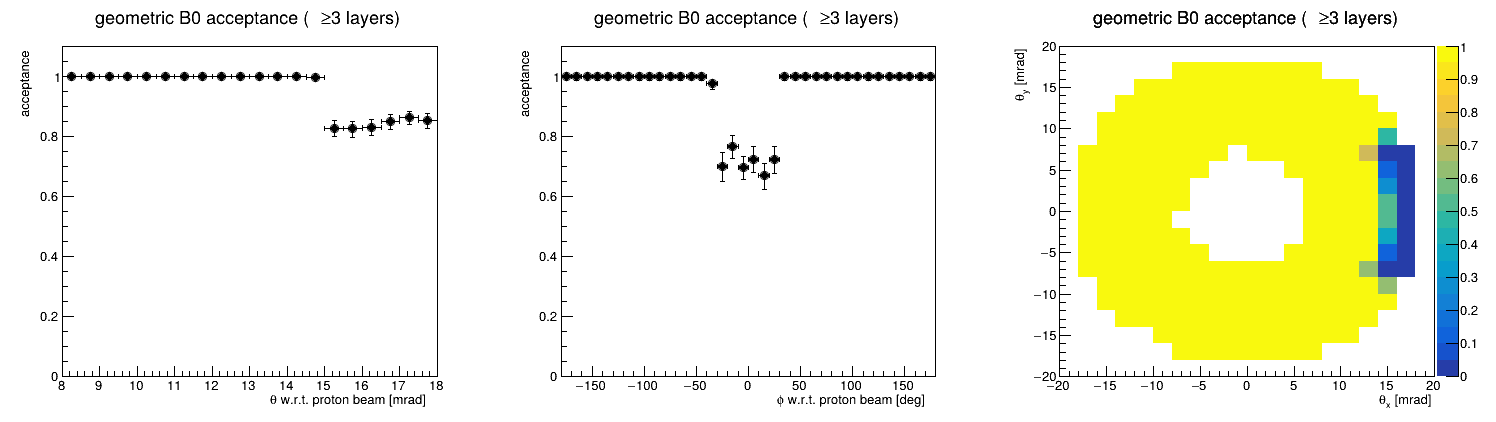
\includegraphics[width=\textwidth]{02_geometric_acceptance/geometric_acceptance_old.png}\\
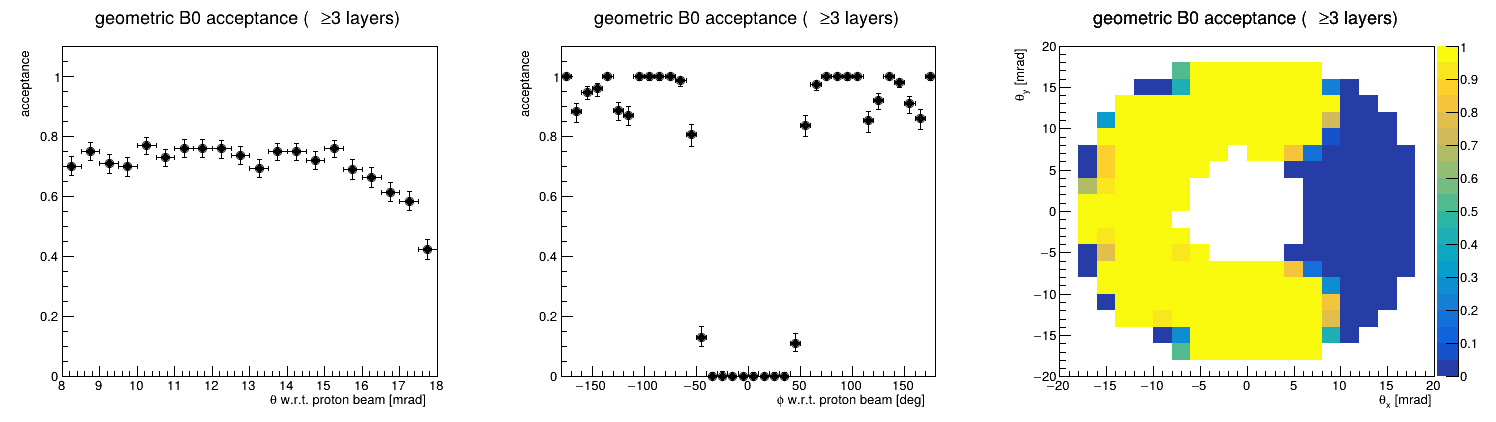
\includegraphics[width=\textwidth]{02_geometric_acceptance/geometric_acceptance_new.png}
\caption{Geometric B0 acceptance ($\ge 3$ layers) for straight lines from the IP (geantinos) vs
$\theta$, $\phi$ and ($\theta_x$, $\theta_y$) w.r.t.\ the proton beam. Top: old geometry; bottom:
new geometry.}
\label{fig:geo}
\end{figure}

Geantinos have no charge and no interactions; ddsim must be run with
\code{--filter.tracker ""} to keep their (zero-energy) hits. Results (5000 events each):
\begin{center}
\begin{tabular}{@{}lcc@{}}
\toprule
& old & new\\
\midrule
$\ge 1$ layer & 95.8\,\% & 83.5\,\%\\
$\ge 3$ layers & \textbf{95.3\,\%} & \textbf{70.1\,\%}\\
4 layers & 93.2\,\% & 66.9\,\%\\
\bottomrule
\end{tabular}
\end{center}
The old geometry covers everything up to 15\,mrad and loses only $\theta > 15$\,mrad on the side
of the electron beam. The new geometry has a gap of about $\pm 45^\circ$ in $\phi$ around
$\phi = 0$ (the electron beam pipe side, $\theta_x \gtrsim +8$\,mrad), where nothing is accepted,
and extra losses above 16\,mrad (Fig.~\ref{fig:geo}).

%=====================================================================================
\section{Acceptance for the $\Lambda$ daughters}

\subsection{Decay kinematics}
The decay releases only 38\,MeV: in the $\Lambda$ rest frame both daughters have
$p^* = 0.1006$\,GeV, with $E^*_p = 0.9435$\,GeV and $E^*_\pi = 0.1723$\,GeV. Boosted to
$p_\Lambda = 50$--$100$\,GeV, both move at nearly the $\Lambda$ velocity and share its momentum
roughly as their rest-frame energies:
\[ \frac{p_p}{p_\Lambda} \approx \frac{E^*_p + p^*\cos\theta^*}{m_\Lambda} \in [0.76, 0.94], \qquad
   \frac{p_\pi}{p_\Lambda} \approx \frac{E^*_\pi - p^*\cos\theta^*}{m_\Lambda} \in [0.06, 0.25], \]
i.e.\ protons of 38--94\,GeV and $\pi^-$ of 3--25\,GeV. The soft $\pi^-$ is bent much more by the
B0 dipole.

\subsection{Results}
\begin{figure}[H]
\centering
\begin{subfigure}{0.78\textwidth}\centering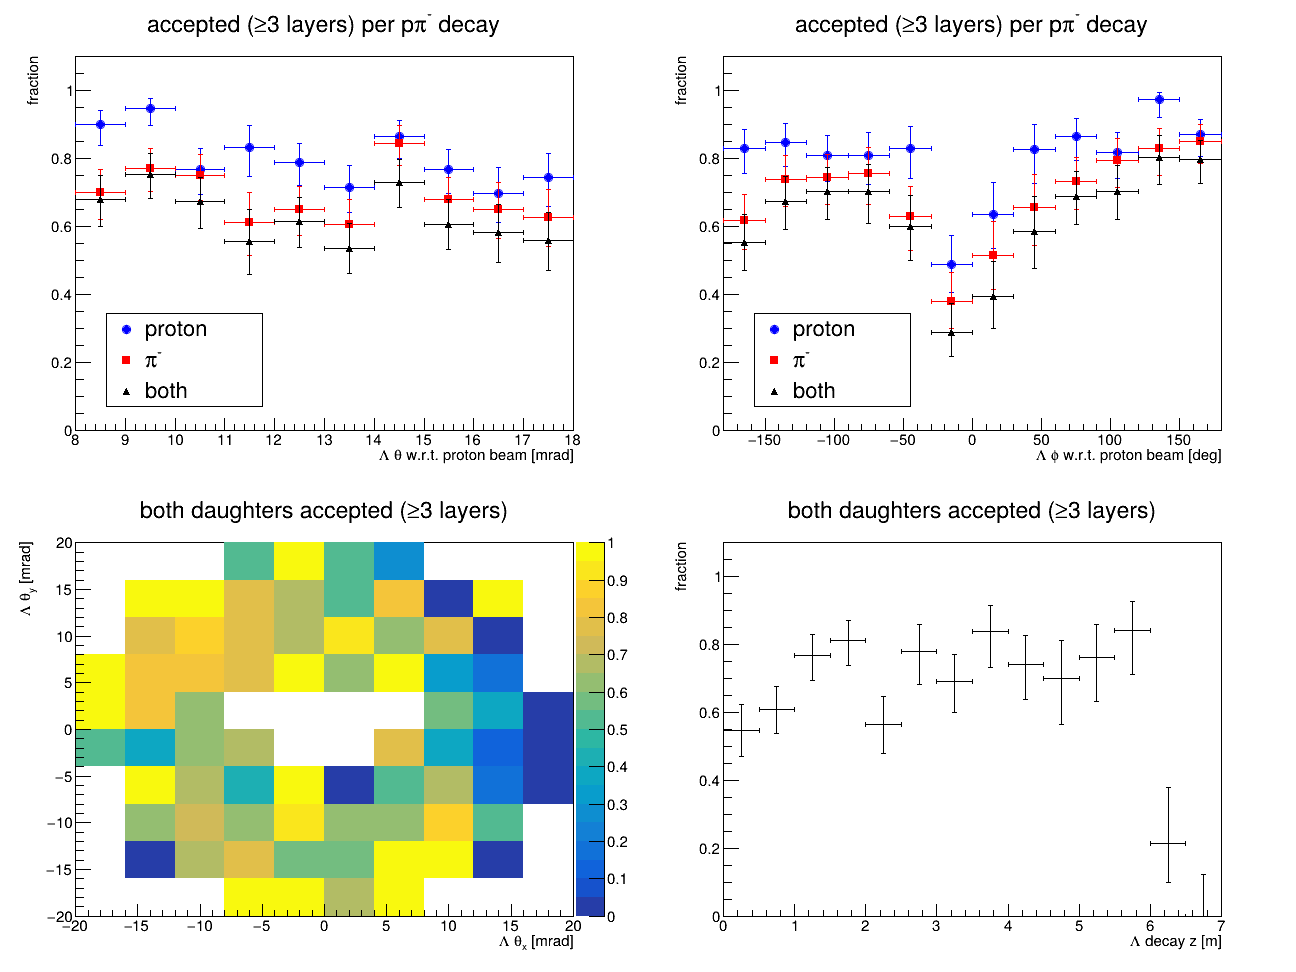
\includegraphics[width=\textwidth]{03_daughter_acceptance/daughter_acceptance_old.png}\caption{old geometry}\end{subfigure}
\begin{subfigure}{0.78\textwidth}\centering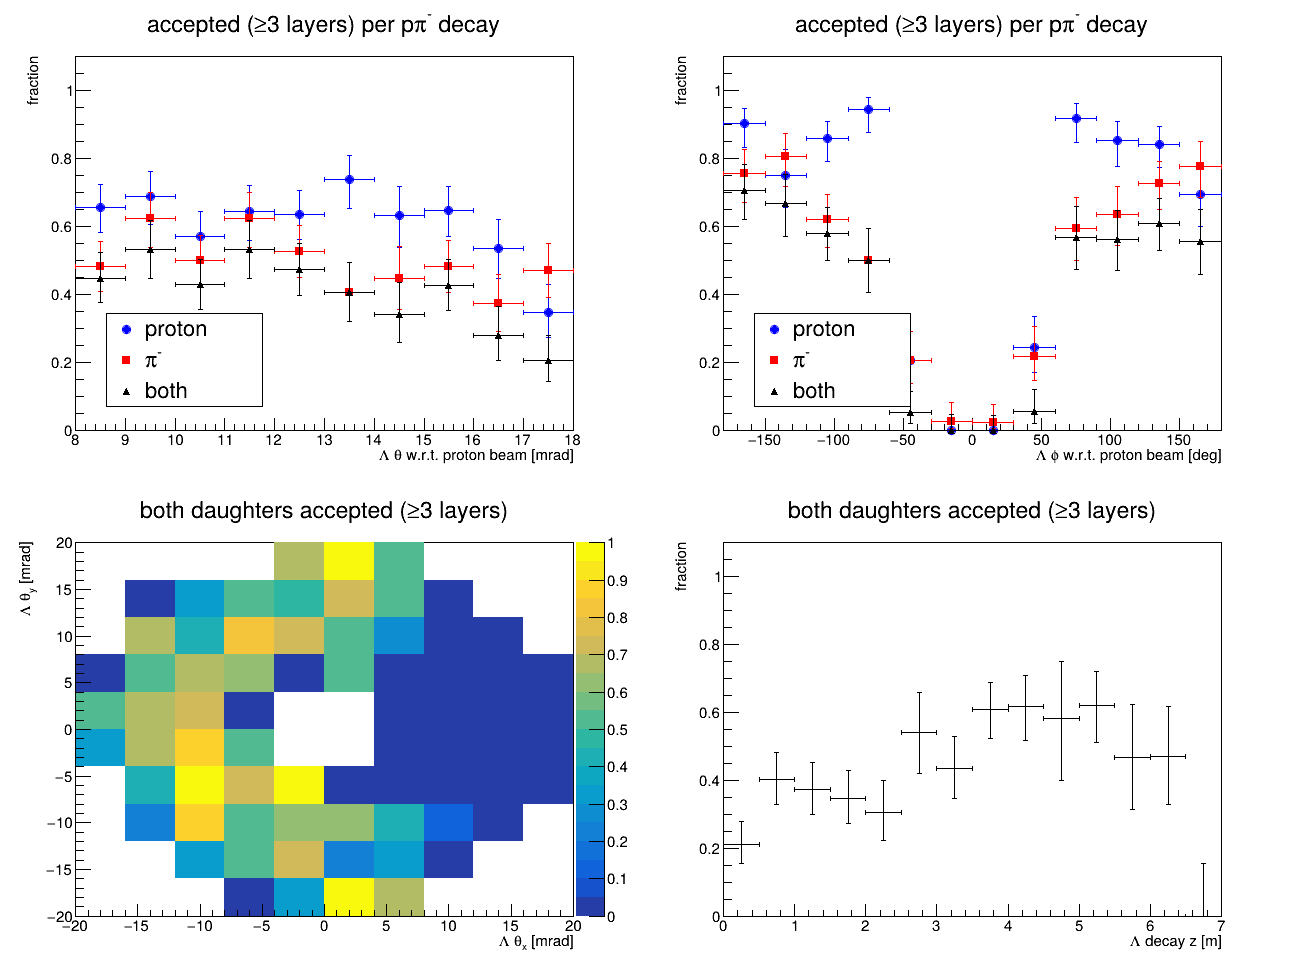
\includegraphics[width=\textwidth]{03_daughter_acceptance/daughter_acceptance_new.png}\caption{new geometry}\end{subfigure}
\caption{Daughter acceptance per $p\pi^-$ decay (proton blue, $\pi^-$ red, both black) vs the
$\Lambda$ $\theta$ and $\phi$, 2D map vs the $\Lambda$ ($\theta_x$, $\theta_y$) for both
daughters, and vs the $\Lambda$ decay $z$. 1000 events per geometry.}
\label{fig:dacc}
\end{figure}

\begin{table}[H]
\centering
\caption{Daughter acceptance per $\Lambda\to p\pi^-$ decay (485--503 decays; statistical error $\approx 2$\,\%).}
\begin{tabular}{@{}lcc@{}}
\toprule
& old geometry & new geometry\\
\midrule
proton, $\ge 3$ layers & 80.3\,\% & 60.8\,\%\\
$\pi^-$, $\ge 3$ layers & 69.4\,\% & 49.5\,\%\\
\textbf{both}, $\ge 3$ layers & \textbf{63.2\,\%} & \textbf{41.0\,\%}\\
both, $\ge 1$ layer & 74.6\,\% & 60.0\,\%\\
both accepted, per generated $\Lambda$ & 31.8\,\% & 19.9\,\%\\
\bottomrule
\end{tabular}
\end{table}

The daughter acceptance is about 30 percentage points below the geometric number: the decay
position, the opening angle between the daughters and the bending of the $\pi^-$ all cost. The
$\phi$ gap of the new geometry is visible as a near-zero acceptance around $\phi = 0$, while the
old geometry only has a dip to 30--40\,\% there. The acceptance rises with the decay distance:
early decays give the daughters more distance to spread away from the $\Lambda$ direction; in the
new geometry only $\approx 20$\,\% of decays near the IP have both daughters accepted. Decays
beyond 6\,m happen inside the tracker and leave too few layers.

%=====================================================================================
\section{Tracking efficiency}

\begin{figure}[H]
\centering
\begin{subfigure}{0.78\textwidth}\centering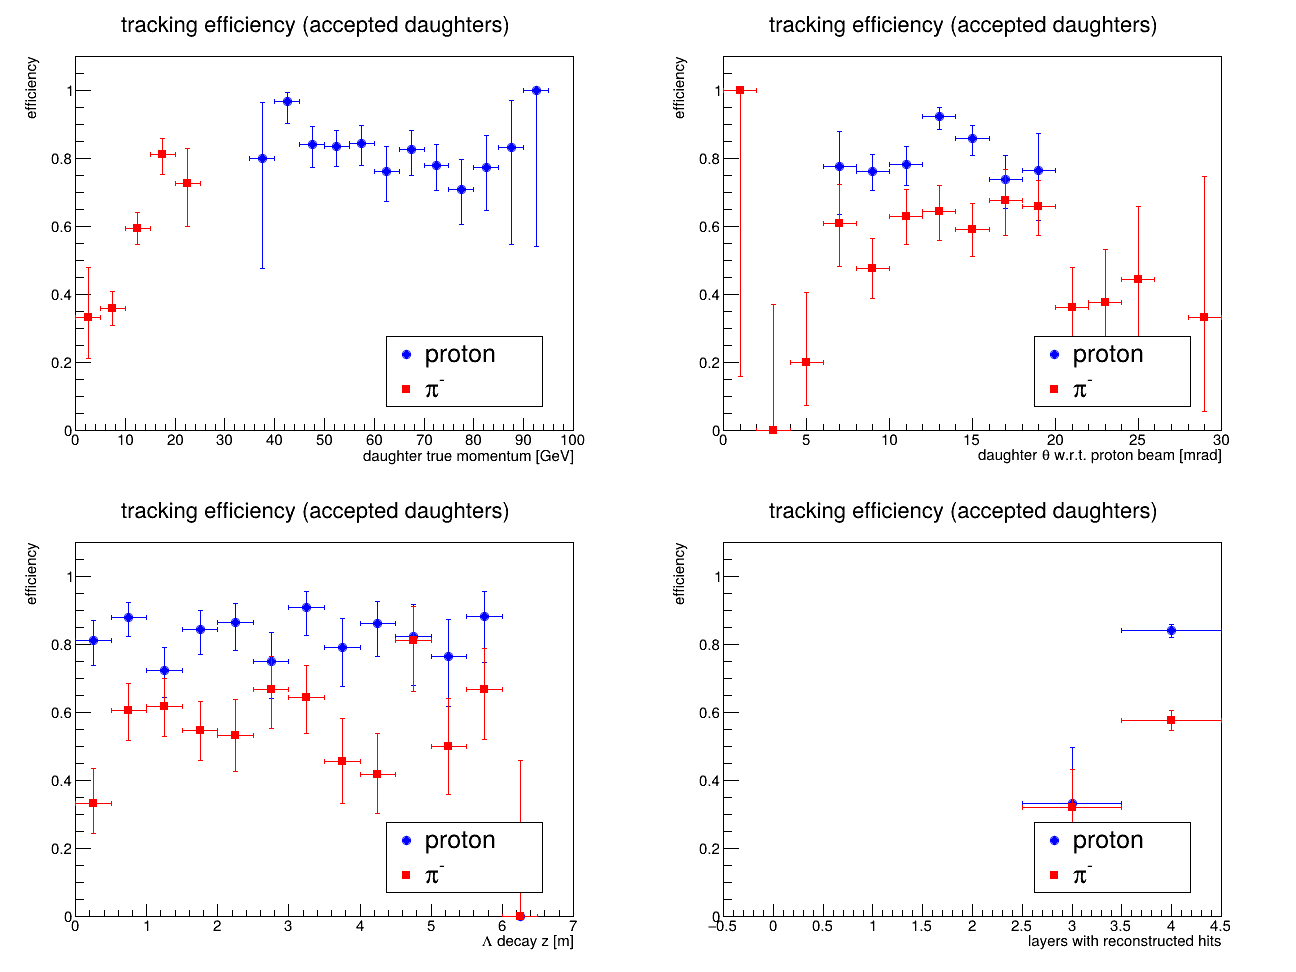
\includegraphics[width=\textwidth]{04_tracking_efficiency/tracking_efficiency_old_10keV.png}\caption{old geometry}\end{subfigure}
\begin{subfigure}{0.78\textwidth}\centering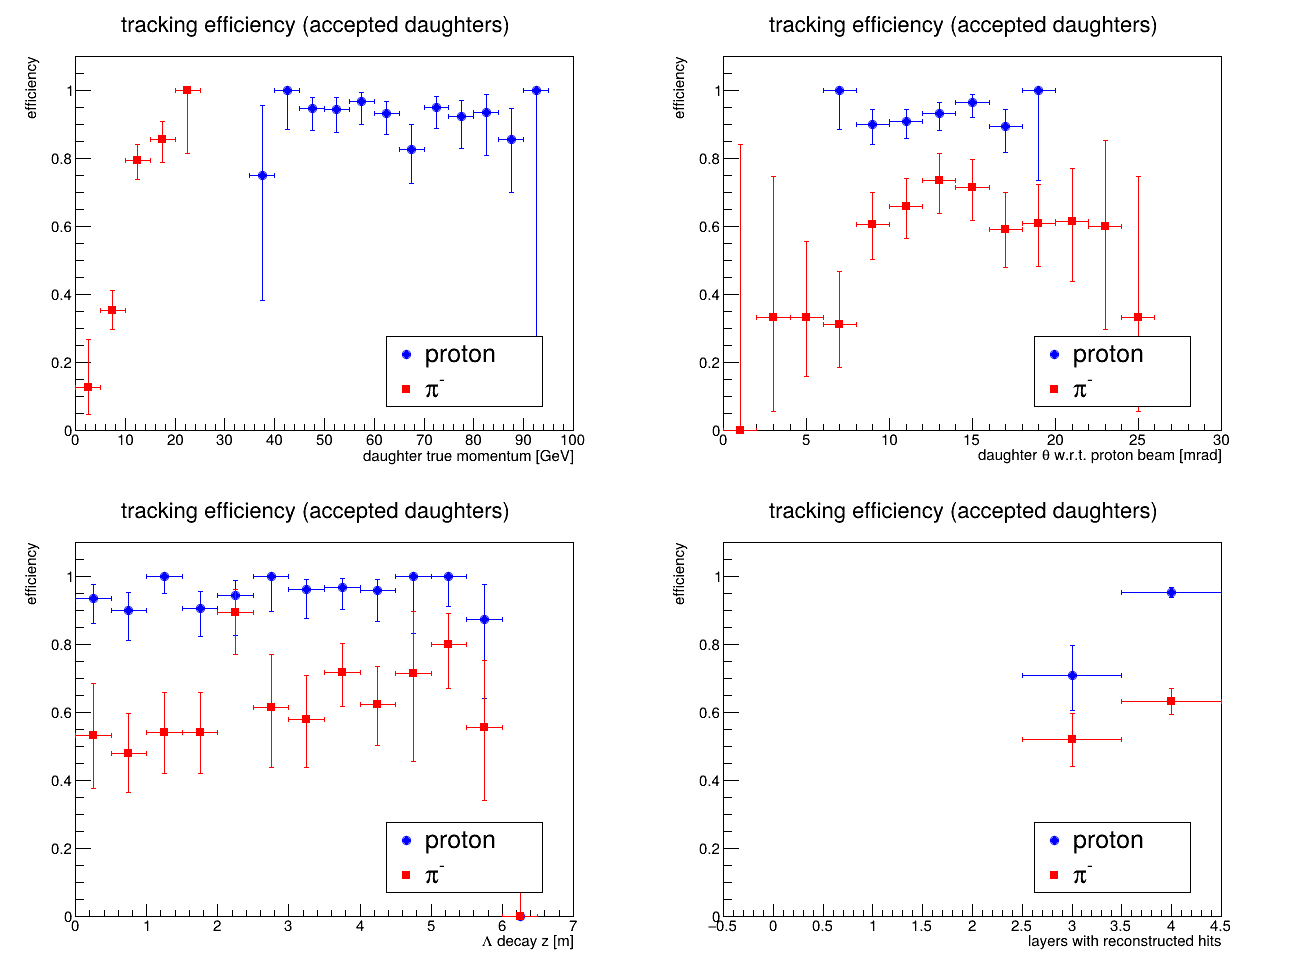
\includegraphics[width=\textwidth]{04_tracking_efficiency/tracking_efficiency_new_5keV.png}\caption{new geometry, 5\,keV}\end{subfigure}
\caption{Tracking efficiency for accepted daughters (proton blue, $\pi^-$ red) vs the daughter's
true momentum, its $\theta$ w.r.t.\ the proton beam, the $\Lambda$ decay $z$, and the number of
layers with reconstructed hits.}
\label{fig:eff}
\end{figure}

\begin{table}[H]
\centering
\caption{Accepted daughters passing each step of the reconstruction (\code{lambda_tracking_efficiency.C}), proton / $\pi^-$. Seeds are matched by charge and direction (they carry no truth link).}
\label{tab:steps}
\begin{tabular}{@{}lccc@{}}
\toprule
step & old geometry & new, 10\,keV & new, 5\,keV\\
\midrule
accepted & 404 / 349 & 295 / 240 & 295 / 240\\
rec.\ hits in $\ge 3$ layers & 100 / 100\,\% & \textbf{93 / 93\,\%} & 100 / 100\,\%\\
seed & 99 / 99\,\% & 97 / 96\,\% & 97 / 96\,\%\\
CKF track & 82 / 56\,\% & 86 / 58\,\% & 93 / 61\,\%\\
filtered track & 82 / 56\,\% & 86 / 58\,\% & 93 / 61\,\%\\
\textbf{reconstructed particle} & \textbf{82.2 / 55.6\,\%} & \textbf{86.1 / 57.5\,\%} & \textbf{92.9 / 60.8\,\%}\\
\bottomrule
\end{tabular}
\end{table}

\paragraph{Where the daughters are lost.} Seeds exist for 96--99\,\% of the accepted daughters; the
loss is entirely in the CKF step (seed $\to$ track). Track filtering and particle building lose
nothing (Table~\ref{tab:steps}).

\paragraph{It is a momentum effect.} The $\pi^-$ efficiency depends strongly on its momentum
(Fig.~\ref{fig:eff}, top left): 12--36\,\% below 10\,GeV, 75--90\,\% at 10--25\,GeV, comparable to
the proton (80--90\,\%, flat over 35--95\,GeV). The $\pi^-$ is low on average only because most
$\pi^-$ are soft. Daughters with reconstructed hits in all four layers are reconstructed more
often than with three.

\paragraph{Seed momentum smearing ruled out.} The truth seeder smears the seed momentum by 10\,\%
(\code{momentumSmear}) and the seed starts at the decay point, often metres before B0 and the
dipole. Rerunning one sample (new geometry, 500 events) with the option
\code{-Ptracking:B0TrackerTruthSeeds:MomentumSmear=0}\\ (verified: seed $q/p$ then equals the true
$q/p$) gives 71 instead of 70 of 120 accepted $\pi^-$ reconstructed: no effect. The cause of the
CKF loss for soft tracks is not identified yet; candidates are the CKF $\chi^2$/measurement cuts,
multiple scattering at low momentum, and the extrapolation of the final track parameters to a
perigee at (0,0,0), a known limitation of EICrecon\#2901.

\subsection{The B0 threshold}
\begin{table}[H]
\centering
\caption{Energy deposited per hit by protons, pions and other non-electron particles (500 events per geometry).}
\begin{tabular}{@{}lcc@{}}
\toprule
& old geometry & new geometry\\
\midrule
sensitive thickness & 300\,$\mu$m & 50\,$\mu$m\\
most probable deposit & 95\,keV & 13.8\,keV\\
hits below 10\,keV & 2.6\,\% & \textbf{9.3\,\%}\\
hits below 5\,keV & 1.6\,\% & 0.3\,\%\\
\bottomrule
\end{tabular}
\end{table}
A minimum-ionizing particle loses $\approx 0.28$\,keV/$\mu$m (most probable) in silicon, so the
50\,$\mu$m sensors give $\approx 14$\,keV, just above the default 10\,keV threshold, which cuts the
low (Landau) tail: 7\,\% of the accepted daughters lose hits and fall below three layers of
reconstructed hits. With 5\,keV (\code{-PB0TRK:B0TrackerRawHits:threshold=5e-6}) all are recovered
and the tracking efficiency of the proton rises from 86\,\% to 93\,\%. In the old geometry the
threshold makes no difference. The 5\,keV setting is not yet the EICrecon default.

%=====================================================================================
\section{Acceptance $\times$ efficiency}

\begin{figure}[H]
\centering
\begin{subfigure}{0.78\textwidth}\centering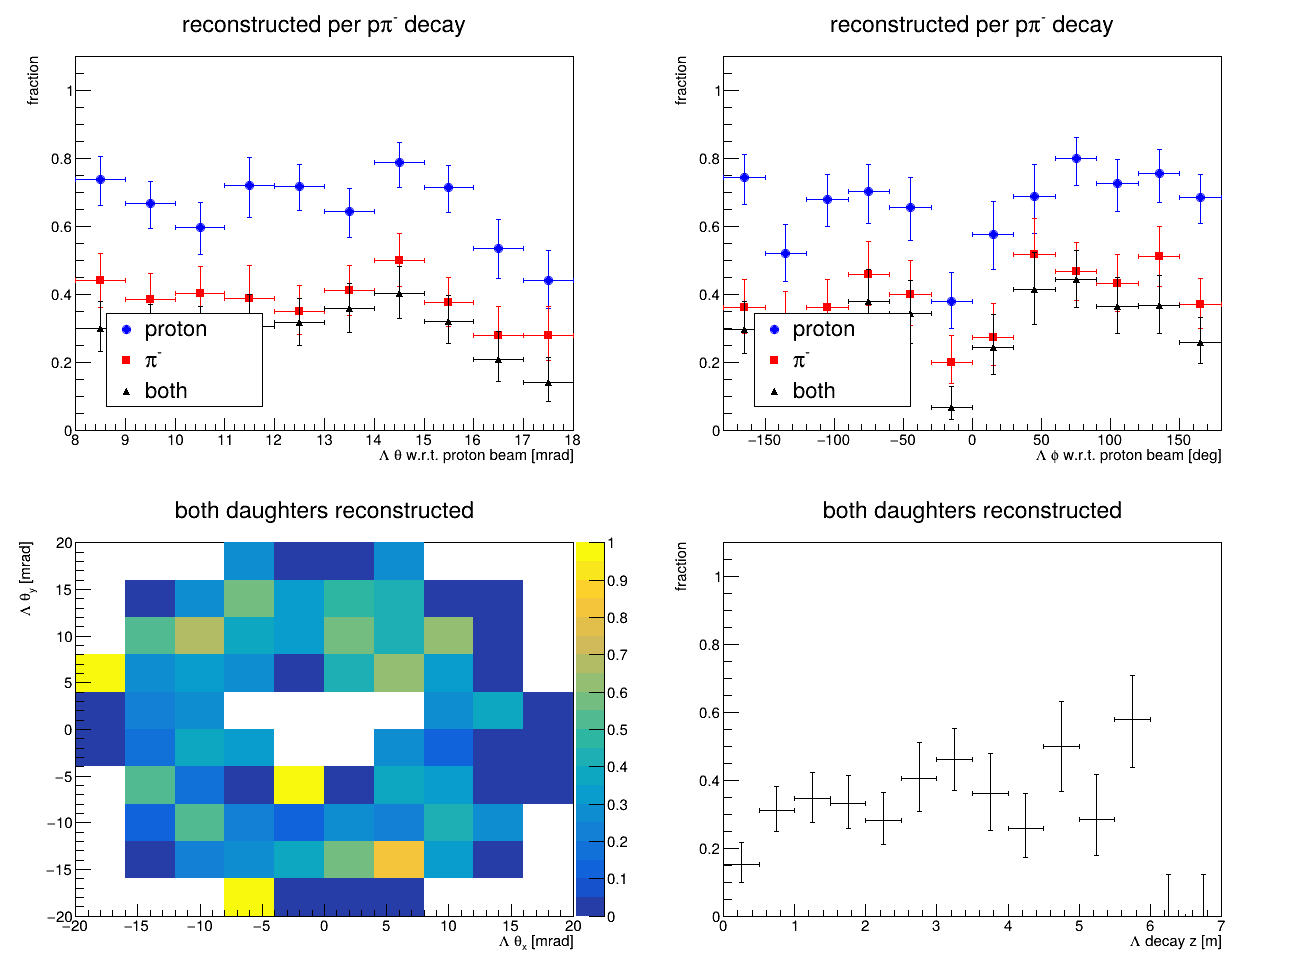
\includegraphics[width=\textwidth]{05_acceptance_x_efficiency/acceptance_x_efficiency_old_10keV.png}\caption{old geometry}\end{subfigure}
\begin{subfigure}{0.78\textwidth}\centering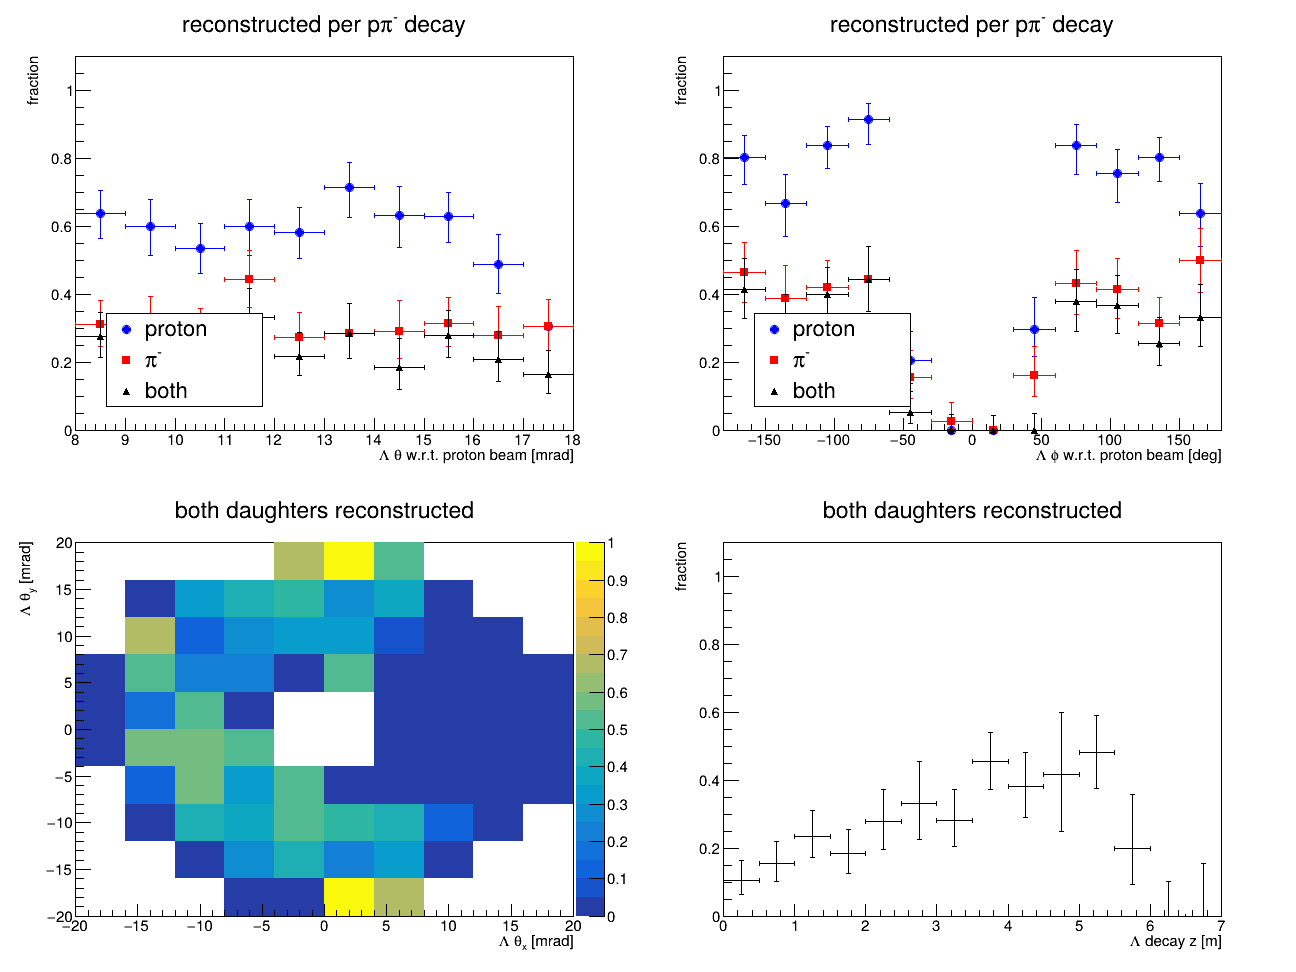
\includegraphics[width=\textwidth]{05_acceptance_x_efficiency/acceptance_x_efficiency_new_5keV.png}\caption{new geometry, 5\,keV}\end{subfigure}
\caption{Acceptance $\times$ efficiency per $p\pi^-$ decay: same panels and denominator as
Fig.~\ref{fig:dacc}, numerator = reconstructed daughters.}
\end{figure}

\begin{table}[H]
\centering
\caption{Acceptance, tracking efficiency and acceptance $\times$ efficiency (\code{lambda_acceptance_x_efficiency.C}), per $p\pi^-$ decay: proton / $\pi^-$ / both.}
\label{tab:axe}
\begin{tabular}{@{}lccc@{}}
\toprule
& old geometry & new, 10\,keV & new, 5\,keV\\
\midrule
acceptance $A$ & 80 / 69 / 63\,\% & 61 / 49 / 41\,\% & 61 / 49 / 41\,\%\\
tracking efficiency $\varepsilon$ & 82 / 56 / 47\,\% & 86 / 58 / 50\,\% & 93 / 61 / 59\,\%\\
$A\times\varepsilon$ & 66 / 39 / \textbf{30\,\%} & 53 / 29 / \textbf{21\,\%} & 57 / 31 / \textbf{25\,\%}\\
\midrule
both reconstructed, per generated $\Lambda$ & \textbf{15.0\,\%} & \textbf{10.1\,\%} & \textbf{12.0\,\%}\\
\bottomrule
\end{tabular}
\end{table}
The direct ratio agrees with the product $A\cdot\varepsilon$ to within 0.6\,\%; at most three
daughters per sample are reconstructed without being accepted. The new geometry at 5\,keV
recovers part of the loss of the new geometry, but stays below the old geometry because of its
smaller acceptance.

%=====================================================================================
\section{The $\Lambda$ mass}

\subsection{Truth-matched pairs}
For each $p\pi^-$ decay with both daughters reconstructed, $M(p\pi^-)$ is computed from the
reconstructed momenta with PDG masses (\code{lambda_mass_reco.C}).
\begin{figure}[H]
\centering
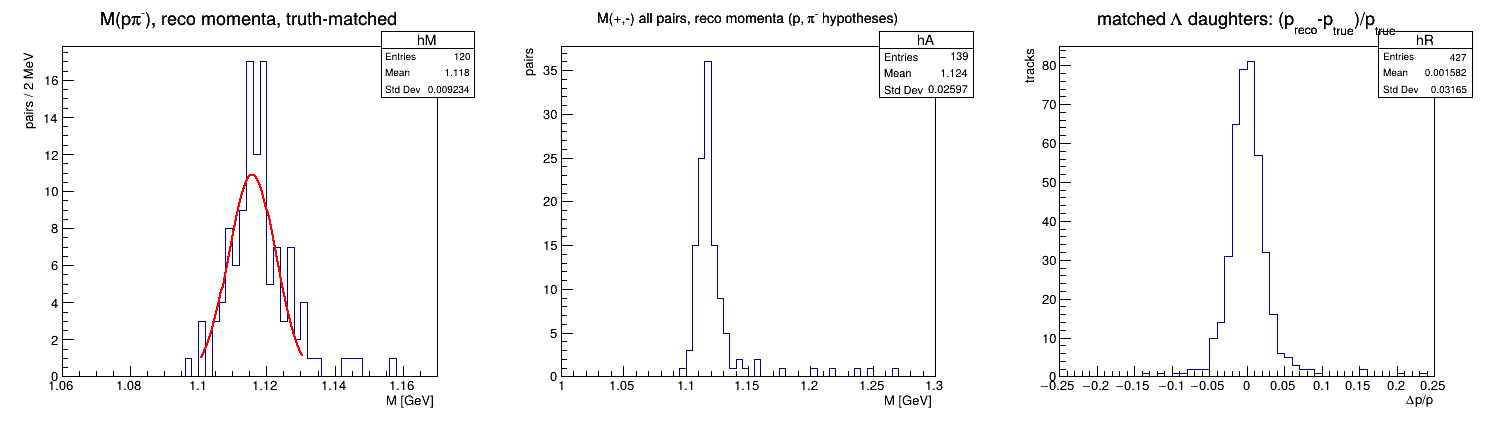
\includegraphics[width=0.9\textwidth]{06_mass/mass_reco_new_5keV.png}
\caption{New geometry, 5\,keV: $M(p\pi^-)$ of truth-matched pairs with a Gaussian fit of the core
(left), all $(+,-)$ pairs without selection (middle), and the momentum resolution of the matched
daughters (right).}
\end{figure}
\begin{table}[H]
\centering
\setlength{\tabcolsep}{4pt}
\begin{tabular}{@{}lccc@{}}
\toprule
& old geometry & new, 10\,keV & new, 5\,keV\\
\midrule
truth-matched pairs (of 1000 $\Lambda$) & 150 & 101 & 120\\
Gaussian mean [GeV] & $1.1177 \pm 0.0007$ & $1.1160 \pm 0.0010$ & $1.1159 \pm 0.0008$\\
Gaussian $\sigma$ [MeV] & $6.3 \pm 0.6$ & $7.4 \pm 1.1$ & $6.9 \pm 1.1$\\
$\Delta p/p$ RMS of matched daughters & 4.4\,\% & 3.2\,\% & 3.2\,\%\\
\bottomrule
\end{tabular}
\end{table}
The new geometry peaks at the PDG mass (1.1157\,GeV). The old geometry is $\approx 2$\,MeV high
($\approx 3\sigma$ of the fit error), not understood. The width is 6--7\,MeV in all samples; the
better momentum resolution of the new geometry does not yet show at this statistics.

\subsection{Without truth in the selection}
Candidates are all $(+,-)$ pairs of reconstructed particles in an event, with the + track as the
proton and the $-$ track as the $\pi^-$. From the kinematics above, $\gamma$ cancels in the
momentum ratio:
\[ r = \frac{p_p}{p_\pi} = \frac{E^*_p + p^*\cos\theta^*}{E^*_\pi - p^*\cos\theta^*}
   \in \left[\frac{0.8429}{0.2729}, \frac{1.0441}{0.0717}\right] = [3.09, 14.6] \]
for any $\Lambda$ momentum, and for an isotropic decay ($\cos\theta^*$ uniform) its distribution
is $f(r) = (E^*_p + E^*_\pi)/[2p^*(1+r)^2]$. The true ratio indeed spans 3.09--14.58 and follows
$f(r)$ (Fig.~\ref{fig:ratio}). The selection $p(+)/p(-) > 2.5$ leaves room for mismeasurement;
it loses $\approx 2$\,\% of the signal (badly measured tracks).

\begin{figure}[H]
\centering
\begin{subfigure}{0.62\textwidth}\centering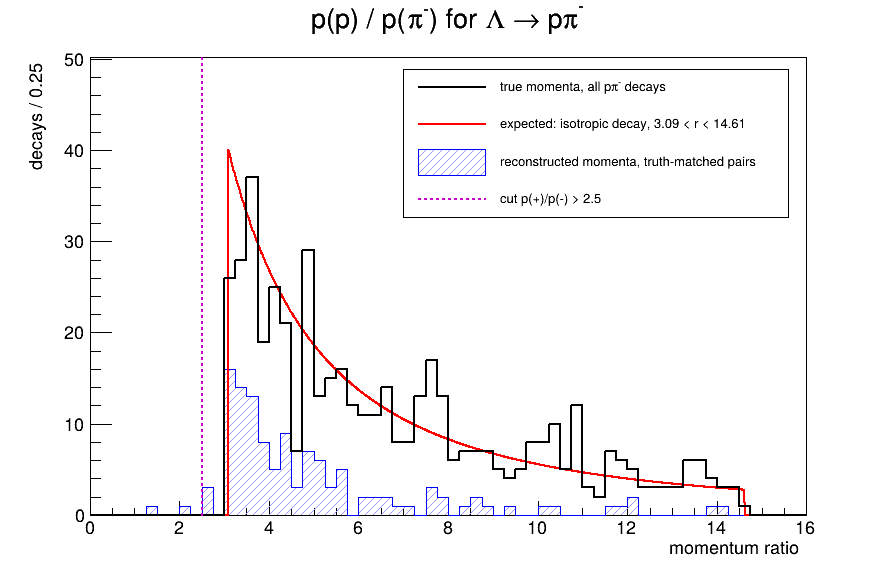
\includegraphics[width=\textwidth]{06_mass/ratio_new_5keV.png}\caption{momentum ratio}\label{fig:ratio}\end{subfigure}
\begin{subfigure}{0.9\textwidth}\centering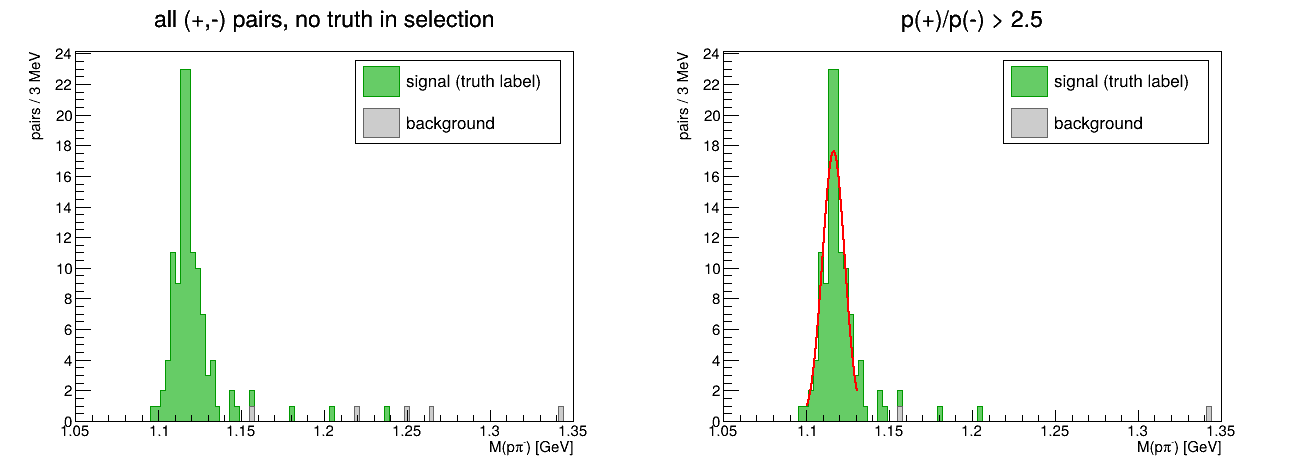
\includegraphics[width=\textwidth]{06_mass/mass_notruth_new_5keV.png}\caption{mass without truth}\end{subfigure}
\caption{New geometry, 5\,keV. (a) True $p(p)/p(\pi^-)$ (black), the expectation for an isotropic
decay (red), and the reconstructed ratio of truth-matched pairs (blue); dashed: the cut.
(b) $M(p\pi^-)$ of all $(+,-)$ pairs (left) and after the cut (right); signal (green, truth label)
stacked on background (grey).}
\end{figure}

\begin{table}[H]
\centering
\setlength{\tabcolsep}{4pt}
\begin{tabular}{@{}lccc@{}}
\toprule
& old geometry & new, 10\,keV & new, 5\,keV\\
\midrule
all $(+,-)$ pairs / purity & 201 / 75\,\% & 116 / 87\,\% & 139 / 86\,\%\\
after $p(+)/p(-)>2.5$ / purity & 155 / \textbf{95\,\%} & 103 / \textbf{96\,\%} & 122 / \textbf{97\,\%}\\
signal kept by the cut & 98\,\% & 98\,\% & 98\,\%\\
$\pm 20$\,MeV window: candidates / signal & 144 / 142 & 92 / 92 & 110 / 110\\
Gaussian mean [GeV] / $\sigma$ [MeV] & 1.1174 / 6.6 & 1.1164 / 6.4 & 1.1166 / 6.7\\
\bottomrule
\end{tabular}
\end{table}
The background (shower tracks, mainly in the old geometry) lies far from the peak. Note that the
tracks are still truth-seeded and the events contain a single $\Lambda$ and nothing else.

%=====================================================================================
\section{Summary and outlook}

\begin{itemize}
\item B0 tracks for displaced $\Lambda$ daughters require the B0 truth seeding of
EICrecon\#2901: 4 $\to$ 77 tracks per 100 $\Lambda$ (old geometry).
\item The realistic B0 geometry (eic/epic\#1194) has a $\pm 45^\circ$ gap in $\phi$ on the
electron-beam side: geometric acceptance 95\,\% $\to$ 70\,\%, daughter acceptance (both)
63\,\% $\to$ 41\,\%.
\item Its 50\,$\mu$m sensors need a 5\,keV threshold (10\,keV loses 7\,\% of the accepted
daughters).
\item Tracking efficiency for accepted daughters: proton 82--93\,\%, $\pi^-$ 56--61\,\%. Soft
tracks ($< 10$\,GeV) are lost in the CKF; not due to the seed momentum smearing.
\item Both daughters reconstructed: 15\,\% (old), 10\,\% (new, 10\,keV), 12\,\% (new, 5\,keV) of
the generated $\Lambda$s.
\item $M(p\pi^-)$ at the PDG value with $\sigma \approx 6$--$7$\,MeV; a single kinematic cut gives
$\approx 97$\,\% purity without truth.
\end{itemize}
Next steps: understand the CKF loss of soft tracks (debug output on a few events, CKF cuts);
realistic B0 seeding (EICrecon\#3028) instead of truth seeding; cross-check with the
ChargedLambdaReconstruction of EICrecon\#2926; the 2\,MeV mass shift in the old geometry; events
with other particles and beam background, where the decay vertex will be needed.

%=====================================================================================
\appendix
\section{Reproducing the results}
\begin{itemize}
\item Builds: \code{scripts/build/build_epic.sh}, \code{scripts/build/build_eicrecon.sh}.
\item Samples: \code{scripts/production/lambda_sample.sh <GEO> <NAME> <SEED> <N>} (simulation,
reconstruction at 10 and 5\,keV, copy to EOS) and \code{scripts/production/geantino_sample.sh}.
\item Analysis: \code{scripts/make_results.sh} runs every macro and writes \code{results/}.
\end{itemize}

\section{Pitfalls met}
\begin{itemize}
\item \code{eic-shell -- bash -c ...} fails (``Illegal option --''); scripts are piped into eic-shell
(\code{scripts/in_eic_shell.sh}), with \code{set --} before sourcing \code{thisepic.sh}.
\item EOS is not visible inside eic-shell: jobs write to the node's \code{/tmp}, then copy.
\item Parallel jobs in one folder can read each other's half-written \code{calibrations/} files.
\item ddsim drops tracker hits below 1\,keV by default (all geantino hits).
\item EICrecon parameters need the plugin prefix (\code{tracking:}, \code{B0TRK:}); an unknown key
stops eicrecon at start-up.
\end{itemize}

\end{document}
